\section{Notation}
\label{app:notation}

Recurring symbols are collected here in order of first appearance.  Each is also
defined at its first use in the text.  Throughout, $\|\cdot\|$ is the Euclidean
norm on vectors and $\|\cdot\|_\op$ the operator norm on matrices.

\begin{longtable}{@{}p{0.20\linewidth}p{0.76\linewidth}@{}}
\toprule
\endfirsthead
\toprule
\endhead
\multicolumn{2}{@{}l}{\emph{Manifold and ambient geometry}}\\
\midrule
$\M$, $k$, $d$ & Embedded $C^3$ manifold without boundary, its dimension, and the ambient dimension, with $1\le k<d$.\\\addlinespace[3pt]
$\T_p\M$, $\N_p\M$ & Tangent and normal spaces at $p\in\M$.\\\addlinespace[3pt]
$U_p$, $U_\perp$ & Matrices with orthonormal columns spanning $\T_p\M$ and $\N_p\M$; $P=U_pU_p^\top$ and $P^\perp=I_d-P$.\\\addlinespace[3pt]
$F_p$, $g_p$, $J_p$ & Normal graph chart at $p$, its normal component, and the area Jacobian $\sqrt{\det(DF_p^\top DF_p)}$.\\\addlinespace[3pt]
$\mathrm{II}_p$, $S_b$, $\mathcal B_a$ & Second fundamental form; shape operator in the normal direction $b$; the map $v\mapsto\mathrm{II}_p[a,v]$.\\\addlinespace[3pt]
$\kappa$ & Curvature of a one-dimensional manifold, used only in Appendix~\ref{app:spiral}.\\\addlinespace[3pt]
$\mathcal T_r$, $\pi$ & Reach tube $\{x:\dist(x,\M)<r\}$ and nearest-point projection onto $\M$.\\\addlinespace[3pt]
\addlinespace
\multicolumn{2}{@{}l}{\emph{Density and its leading jet}}\\
\midrule
$\mu$, $\rho$ & Law of the clean variable $X$ and its density with respect to Riemannian volume.\\\addlinespace[3pt]
$a_p$ & Effective chart density $\rho(F_p(z))J_p(z)$, whose jets drive every limit.\\\addlinespace[3pt]
$q_m$, $m$ & First nonzero homogeneous jet of $a_p$ and its degree, the vanishing order.\\\addlinespace[3pt]
$\mathcal Z_q$, $C_{q_m}$ & Normalizer $\int q_me^{-\|u\|^2/2}du$ and the covariance \eqref{eq:Cq} of the $q_m$-tilted Gaussian.\\\addlinespace[3pt]
\addlinespace
\multicolumn{2}{@{}l}{\emph{Noise, score and denoiser}}\\
\midrule
$\sigma$, $Y_\sigma$, $p_\sigma$ & Noise scale, the observation $X+\sigma G$, and its density.\\\addlinespace[3pt]
$s_\sigma$, $D_\sigma$, $H_\sigma$ & Score $\nabla\log p_\sigma$, denoiser $y+\sigma^2s_\sigma$, and link Hessian $\nabla D_\sigma=\sigma^{-2}\Cov(X\mid Y_\sigma=y)$.\\\addlinespace[3pt]
$s_\theta$, $\widehat A_\theta$ & Learned score and its symmetrized link Jacobian.\\\addlinespace[3pt]
\addlinespace
\multicolumn{2}{@{}l}{\emph{Spectral calibration}}\\
\midrule
$A_0$, $c_q$ & Limiting operator $U_pC_{q_m}U_p^\top$ and its smallest nonzero eigenvalue $\lambda_{\min}(C_{q_m})$.\\\addlinespace[3pt]
$\mathcal P_k$, $Q_\sigma$ & Orthogonal projector onto a top-$k$ eigenspace, and $\mathcal P_k(H_\sigma)$.\\\addlinespace[3pt]
$\eta$, $\delta(\widehat A)$ & Operator-norm estimation error $\|\widehat A-A_0\|_\op$ and the computed separation \eqref{eq:computed-separation}.\\\addlinespace[3pt]
$\vartheta_{\mathrm{sp}}$, $\tau$, $\Phi_\tau$ & Hard spectral cutoff, soft filter strength, and the filter $\widehat A(\widehat A+\tau I)^{-1}$.\\\addlinespace[3pt]
\addlinespace
\multicolumn{2}{@{}l}{\emph{Boundary layer at a finite-type point}}\\
\midrule
$a$, $b$ & Rescaled tangential and normal coordinates of a query, so the query is $F_p(\sigma a)+\sigma b$.\\\addlinespace[3pt]
$\nu_{q,a}$, $C_a$, $\mu_a$ & Shifted tilted law with density $\propto q_m(a+u)e^{-\|u\|^2/2}$, its covariance and its mean.\\\addlinespace[3pt]
$\Gamma_a$, $\Lambda_a$ & Normal-valued covariance \eqref{eq:normal-boundary-objects} and its calibrated version $\Gamma_aC_a^{-1}$.\\\addlinespace[3pt]
$K_T$, $K_N$, $c_0$ & Compact sets of admissible $a$ and $b$, and $\inf_{a\in K_T}\lambda_{\min}(C_a)$.\\\addlinespace[3pt]
\addlinespace
\multicolumn{2}{@{}l}{\emph{Optimization}}\\
\midrule
$f$, $F$, $\gamma$ & Ambient objective, its pullback $f\circ\pi$, and the step size.\\\addlinespace[3pt]
$L$, $Q$, $\overline D_Q$ & Landing map, tangent projector oracle, and the normal-only landing \eqref{eq:normal-landing}.\\\addlinespace[3pt]
$\eps_P$, $\eps_L$ & Oracle errors of Assumption~\ref{ass:oracles}, for the projector and the landing map.\\\addlinespace[3pt]
$\beta_H$, $\beta_L$, $g_\sigma$ & Population Jacobian bias, population landing bias, and tangent-normal eigengap, all defined in Corollary~\ref{cor:learned}.\\\addlinespace[3pt]
$\eps_s$, $\eps_J$, $R_D$ & Uniform score error, score-Jacobian error, and a bound on $\|D_\sigma(y)-y\|$.\\\addlinespace[3pt]
$\mathcal V$ & Query set containing every iterate $x_t$ and intermediate point $z_t$.\\\addlinespace[3pt]
$B$, $L_f$, $L_F$, $L_\pi$, $K_\pi$ & Gradient bound and Lipschitz constants of $\nabla f$, $\nabla F$, $\pi$ and $\mathrm d\pi$.\\\addlinespace[3pt]
$G_f$ & Tangent block $U_p^\top\nabla^2f(p)U_p$ of the ambient Hessian.\\\addlinespace[3pt]
\bottomrule
\end{longtable}

\section{Exact posterior identities}
\label{app:tweedie}

For Proposition~\ref{prop:tweedie}, let
\[
  \varphi_\sigma(y-x)
  =(2\pi\sigma^2)^{-d/2}
  \exp\!\left(-\frac{\|y-x\|^2}{2\sigma^2}\right).
\]
The Gaussian factor and all of its derivatives are bounded as functions of $x$ for fixed $\sigma>0$.  Since $\mu$ is finite, differentiation under the integral is justified by dominated convergence.  We obtain
\begin{align}
  \nabla p_\sigma(y)
  &=\int \frac{x-y}{\sigma^2}\varphi_\sigma(y-x)\,\mu(dx),\\
  \nabla\log p_\sigma(y)
  &=\frac{\E[X\mid Y_\sigma=y]-y}{\sigma^2}.
\end{align}
This is the posterior-mean identity.

To differentiate the conditional mean, write $m(y)=\E[X\mid Y_\sigma=y]$.  In coordinates,
\begin{align}
  \partial_{y_j}m_i(y)
  &=
  \frac{1}{\sigma^2}
  \left(
  \E[X_iX_j\mid Y_\sigma=y]
  -\E[X_i\mid Y_\sigma=y]\E[X_j\mid Y_\sigma=y]
  \right).
\end{align}
Therefore $\nabla m(y)=\sigma^{-2}\Cov(X\mid Y_\sigma=y)$.  Since $m=D_\sigma$, differentiating \eqref{eq:link} proves the second identity and symmetry of $H_\sigma$.

\section{A localized Laplace expansion}
\label{app:laplace}

In the normal graph \eqref{eq:chart}, assume
\begin{align}
  g_p(z)&=\tfrac12\mathrm{II}_p[z,z]+R_g(z),
  &\|R_g(z)\|&\le C\|z\|^3,\label{eq:normal-exp}\\
  a_p(z)&=q_m(z)+q_{m+1}(z)+R_a(z),
  &|R_a(z)|&\le C\|z\|^{m+2}.\label{eq:density-exp-app}
\end{align}
Here $\mathrm{II}_p:\R^k\times\R^k\to\N_p\M$ is the second fundamental form in the chosen frame.  The normal graph is orthogonal to $U_pz$, so
\begin{equation}
  \|F_p(z)-p\|^2=\|z\|^2+\|g_p(z)\|^2
  =\|z\|^2+O(\|z\|^4).
  \label{eq:distance-exp}
\end{equation}

Choose the chart so that $\M\cap B(p,\eta)$ is contained in its image.  The contribution from $\M\setminus B(p,\eta)$ to a posterior moment of order $s\in\{0,1,2\}$ is at most
\begin{equation}
  O\!\left(e^{-\eta^2/(4\sigma^2)}\right),
  \label{eq:tail-localization}
\end{equation}
after absorbing a bounded polynomial factor into the exponential.  This term is smaller than every power of $\sigma$.

Inside the chart set $z=\sigma u$.  For $\|u\|<\eta/\sigma$,
\begin{align}
  \sigma^{-m}a_p(\sigma u)
  &=q_m(u)+\sigma q_{m+1}(u)
    +O(\sigma^2\|u\|^{m+2}),\label{eq:density-scale}\\
  \exp\!\left(-\frac{\|g_p(\sigma u)\|^2}{2\sigma^2}\right)
  &=1+O(\sigma^2\|u\|^4).\label{eq:kernel-scale}
\end{align}
The expansion \eqref{eq:kernel-scale} is to be read on bounded sets of $u$; on the whole chart, where $\|u\|$ may reach $\eta/\sigma$, the elementary bound $|e^{-t}-1|\le t$ for $t\ge0$ gives instead $0\le1-\exp(-\|g_p(\sigma u)\|^2/2\sigma^2)\le C\sigma^2\|u\|^4$ with the same constant, and $\|g_p(\sigma u)\|\le C\sigma^2\|u\|^2$ makes the exponent nonnegative, so the factor never exceeds one.  On a smaller fixed chart, these remainders are dominated by a polynomial in $\|u\|$ times $e^{-c\|u\|^2}$.  The annulus between that smaller chart and the original one is exponentially negligible.  Dominated convergence therefore permits termwise integration over $\R^k$.

Let
\[
  \mathcal Z_q=\int_{\R^k}q_m(u)e^{-\|u\|^2/2}\,du
  =(2\pi)^{k/2}\,\E[q_m(Z)],\qquad Z\sim\cN(0,I_k).
\]
The unnormalized $\mathcal Z_q$ and the expectation $\E[q_m(Z)]$ used in
\eqref{eq:Cq} therefore differ by the Gaussian normalizing constant, which
cancels in every ratio below.  Because $q_m$ is even and $q_{m+1}$ is odd,
\begin{equation}
  \int_\M e^{-\|x-p\|^2/(2\sigma^2)}\,\mu(dx)
  =\sigma^{k+m}\bigl(\mathcal Z_q+O(\sigma^2)\bigr).
  \label{eq:normalizer-exp}
\end{equation}
The order-$\sigma$ term vanishes by parity.  Multiplication by the ambient Gaussian normalization gives
\begin{equation}
  p_\sigma(p)
  =(2\pi)^{-d/2}\mathcal Z_q\,
  \sigma^{k+m-d}\bigl(1+O(\sigma^2)\bigr).
  \label{eq:noisy-density-scaling}
\end{equation}
The smoothed-density power law therefore contains the vanishing order.

\section{Proof of the finite-type theorem}
\label{app:finite-proof}

\subsection{Parity and positivity}

For every fixed $u$,
\[
  q_m(u)=\lim_{t\downarrow0}\frac{a_p(tu)}{t^m}\ge0.
\]
If $m$ were odd, homogeneity would give $q_m(-u)=-q_m(u)$.  Nonnegativity in both directions would imply $q_m\equiv0$, a contradiction.  Hence $m$ is even, $q_m$ is even, and it is positive on some nonempty open set.  In particular $\mathcal Z_q>0$.

\subsection{Posterior mean}

Let $N_1$ denote the unnormalized first centered moment about $p$.  Its tangent component is
\begin{align}
  P_{\T_p\M}N_1
  &=
  U_p\sigma^{k+m+1}
  \int_{\R^k}u
  \bigl(q_m(u)+\sigma q_{m+1}(u)+O(\sigma^2\operatorname{poly}(u))\bigr)
  e^{-\|u\|^2/2}\,du\nonumber\\
  &=
  U_p\sigma^{k+m+2}
  \int_{\R^k}u q_{m+1}(u)e^{-\|u\|^2/2}\,du
  +O(\sigma^{k+m+3}).
  \label{eq:tangent-first}
\end{align}
The leading integral vanishes because $u q_m(u)$ is odd.  From \eqref{eq:normal-exp}, the normal component is
\begin{equation}
  P_{\N_p\M}N_1
  =
  \frac{\sigma^{k+m+2}}{2}
  \int_{\R^k}\mathrm{II}_p[u,u]q_m(u)e^{-\|u\|^2/2}\,du
  +O(\sigma^{k+m+3}).
  \label{eq:normal-first}
\end{equation}
Dividing \eqref{eq:tangent-first} and \eqref{eq:normal-first} by \eqref{eq:normalizer-exp} yields \eqref{eq:meanlimit}, with
\begin{equation}
  b_{p,q}
  =
  U_p\frac{\int u q_{m+1}(u)e^{-\|u\|^2/2}\,du}{\mathcal Z_q}
  +\frac12
  \frac{\int \mathrm{II}_p[u,u]q_m(u)e^{-\|u\|^2/2}\,du}{\mathcal Z_q}.
  \label{eq:b-explicit}
\end{equation}

\subsection{Posterior covariance}

Write $N_0$ for the normalizer \eqref{eq:normalizer-exp} and $N_2$ for the
unnormalized second moment about $p$,
\begin{equation}
  N_0=\int_\M e^{-\|x-p\|^2/(2\sigma^2)}\mu(dx),
  \qquad
  N_2=\int_\M(x-p)(x-p)^\top e^{-\|x-p\|^2/(2\sigma^2)}\mu(dx),
  \label{eq:n0-n2}
\end{equation}
so that $\E[(X-p)(X-p)^\top\mid Y_\sigma=p]=N_2/N_0$.  We compute the three
blocks of $N_2$ and then divide.

In the chart, $\mu(dx)=a_p(z)\,dz$ and $z=\sigma u$ gives $dz=\sigma^k du$, while
\eqref{eq:distance-exp} splits the kernel as
\begin{equation}
  e^{-\|F_p(\sigma u)-p\|^2/(2\sigma^2)}
  =e^{-\|u\|^2/2}\,
   \exp\!\left(-\frac{\|g_p(\sigma u)\|^2}{2\sigma^2}\right)
  =e^{-\|u\|^2/2}\bigl(1+O(\sigma^2\|u\|^4)\bigr),
  \label{eq:kernel-split}
\end{equation}
by \eqref{eq:kernel-scale}.  Combining this with \eqref{eq:density-scale}, the
unnormalized measure element is
\begin{equation}
  a_p(\sigma u)\,\sigma^k\,e^{-\|F_p(\sigma u)-p\|^2/(2\sigma^2)}\,du
  =\sigma^{k+m}
   \Bigl(q_m(u)+\sigma q_{m+1}(u)+O\bigl(\sigma^2\operatorname{poly}(u)\bigr)\Bigr)
   e^{-\|u\|^2/2}\,du,
  \label{eq:measure-element}
\end{equation}
the kernel remainder of \eqref{eq:kernel-split} having been absorbed into the
$O(\sigma^2\operatorname{poly}(u))$ term.  The displacement itself splits as
\begin{equation}
  x-p=U_p(\sigma u)+g_p(\sigma u),
  \qquad
  g_p(\sigma u)=\frac{\sigma^2}{2}\mathrm{II}_p[u,u]+O(\sigma^3\|u\|^3),
  \label{eq:displacement-split}
\end{equation}
using \eqref{eq:normal-exp}.

\emph{Tangent-tangent block.}  The tangent part of \eqref{eq:displacement-split}
contributes $\sigma^2U_puu^\top U_p^\top$, so by \eqref{eq:measure-element}
\begin{align}
  P_{\T_p\M}N_2P_{\T_p\M}
  &=\sigma^{k+m+2}U_p
    \int_{\R^k}uu^\top
    \Bigl(q_m(u)+\sigma q_{m+1}(u)+O\bigl(\sigma^2\operatorname{poly}(u)\bigr)\Bigr)
    e^{-\|u\|^2/2}\,du\;U_p^\top\nonumber\\
  &=\sigma^{k+m+2}U_p
    \left(\int_{\R^k}uu^\top q_m(u)e^{-\|u\|^2/2}\,du
    +O(\sigma^2)\right)U_p^\top.
  \label{eq:tt-second}
\end{align}
The order-$\sigma$ term drops because $uu^\top q_{m+1}(u)$ is odd, $uu^\top$
being even and $q_{m+1}$ odd.  The surviving integral is exactly
$\mathcal Z_qC_{q_m}$: writing $Z\sim\cN(0,I_k)$,
\begin{equation}
  \int_{\R^k}uu^\top q_m(u)e^{-\|u\|^2/2}\,du
  =(2\pi)^{k/2}\,\E\bigl[ZZ^\top q_m(Z)\bigr]
  =(2\pi)^{k/2}\,\E[q_m(Z)]\,C_{q_m}
  =\mathcal Z_qC_{q_m},
  \label{eq:tt-integral}
\end{equation}
where the middle step is the definition \eqref{eq:Cq} of $C_{q_m}$ and the last
is the definition of $\mathcal Z_q$.  Hence
\begin{equation}
  P_{\T_p\M}N_2P_{\T_p\M}
  =\sigma^{k+m+2}\mathcal Z_q
   \bigl(U_pC_{q_m}U_p^\top+O(\sigma^2)\bigr).
  \label{eq:tt-final}
\end{equation}

\emph{Tangent-normal block.}  Pairing the tangent part of
\eqref{eq:displacement-split} with the normal part gives a prefactor
$\sigma\cdot\sigma^2/2$, so
\begin{align}
  P_{\T_p\M}N_2P_{\N_p\M}
  &=\frac{\sigma^{k+m+3}}{2}U_p
    \int_{\R^k}u\,\mathrm{II}_p[u,u]^\top q_m(u)e^{-\|u\|^2/2}\,du
    +O(\sigma^{k+m+4})\nonumber\\
  &=O(\sigma^{k+m+4}).
  \label{eq:tn-second}
\end{align}
The displayed integral vanishes by parity: $u$ is odd while
$\mathrm{II}_p[u,u]$ and $q_m(u)$ are both even, so the integrand is odd.  The
nominal order-$\sigma^{k+m+3}$ term is therefore absent, and what remains comes
from the $O(\sigma^3\|u\|^3)$ remainder in \eqref{eq:displacement-split} and from
the $\sigma q_{m+1}$ term in \eqref{eq:measure-element}.

\emph{Normal-normal block.}  Both factors are normal, so by
\eqref{eq:displacement-split} the integrand carries $\|g_p(\sigma u)\|^2
=O(\sigma^4\|u\|^4)$ and
\begin{equation}
  P_{\N_p\M}N_2P_{\N_p\M}=O(\sigma^{k+m+4}).
  \label{eq:nn-second}
\end{equation}

\emph{Division and centering.}  Assembling \eqref{eq:tt-final},
\eqref{eq:tn-second} and \eqref{eq:nn-second}, and dividing by
$N_0=\sigma^{k+m}(\mathcal Z_q+O(\sigma^2))$ from \eqref{eq:normalizer-exp},
\begin{equation}
  \E\bigl[(X-p)(X-p)^\top\mid Y_\sigma=p\bigr]
  =\frac{N_2}{N_0}
  =\frac{\sigma^{k+m+2}\mathcal Z_q\bigl(U_pC_{q_m}U_p^\top+O(\sigma^2)\bigr)}
        {\sigma^{k+m}\bigl(\mathcal Z_q+O(\sigma^2)\bigr)}
  =\sigma^2U_pC_{q_m}U_p^\top+O(\sigma^4),
  \label{eq:second-moment-final}
\end{equation}
where the last step uses $\mathcal Z_q>0$ from Appendix~\ref{app:finite-proof}
and expands $(\mathcal Z_q+O(\sigma^2))^{-1}=\mathcal Z_q^{-1}(1+O(\sigma^2))$.
Finally $\eqref{eq:meanlimit}$ gives
$\E[X\mid Y_\sigma=p]-p=\sigma^2b_{p,q}+O(\sigma^3)$, so subtracting the outer
product of the mean removes only an $O(\sigma^4)$ matrix:
\begin{equation}
  \Cov(X\mid Y_\sigma=p)
  =\sigma^2U_pC_{q_m}U_p^\top+O(\sigma^4).
  \label{eq:cov-final}
\end{equation}
Dividing by $\sigma^2$ and applying Proposition~\ref{prop:tweedie} proves
\eqref{eq:hlimit}.

\subsection{Rank and trace}

For $v\ne0$,
\begin{equation}
  v^\top C_{q_m}v
  =
  \frac{\int(v^\top u)^2q_m(u)e^{-\|u\|^2/2}\,du}
  {\mathcal Z_q}>0.
\end{equation}
The strict inequality holds because $q_m$ is positive on an open set, which cannot be contained in the hyperplane $v^\top u=0$.  Hence $C_{q_m}\succ0$, and the ambient limit has rank $k$ and range $\T_p\M$.

Euler's identity gives $u^\top\nabla q_m(u)=m q_m(u)$.  Integrating the divergence of $u q_m(u)e^{-\|u\|^2/2}$ gives
\begin{align}
  0
  &=
  \int_{\R^k}
  \bigl(kq_m(u)+u^\top\nabla q_m(u)-\|u\|^2q_m(u)\bigr)
  e^{-\|u\|^2/2}\,du\\
  &=
  \int_{\R^k}
  \bigl(k+m-\|u\|^2\bigr)q_m(u)e^{-\|u\|^2/2}\,du.
\end{align}
Dividing by $\mathcal Z_q$ proves $\tr C_{q_m}=k+m$.

\subsection{Positive density and change of tangent frame}

If $\rho(p)>0$, then the first jet is the positive constant
$q_0=\rho(p)$ (the chart volume factor equals one at the origin).  Its
Gaussian tilt is unchanged, so $C_{q_0}=\E[ZZ^\top]=I_k$ and
$U_pC_{q_0}U_p^\top=P_{\T_p\M}$.

For coordinate invariance, let $\widetilde U_p=U_pO$ for $O\in O(k)$.
The same density jet in the new coordinates is
$\widetilde q_m(\widetilde z)=q_m(O\widetilde z)$.  Rotational invariance of
the standard Gaussian gives
\[
  C_{\widetilde q_m}=O^\top C_{q_m}O.
\]
It follows that
$\widetilde U_pC_{\widetilde q_m}\widetilde U_p^\top
=U_pC_{q_m}U_p^\top$, proving Corollary~\ref{cor:regular}.

\subsection{Minimal assumptions and rate assumptions}

The operator limit requires less regularity than the stated rate.  If
$g_p(z)=o(\|z\|)$ and $a_p(z)=q_m(z)+o(\|z\|^m)$, dominated convergence in the rescaled posterior gives
\[
  \sigma^{-2}\Cov(X\mid Y_\sigma=p)\to U_pC_{q_m}U_p^\top.
\]
For $D_\sigma(p)-p=O(\sigma^2)$ it suffices that $g_p(z)=O(\|z\|^2)$ and
$a_p(z)=q_m(z)+O(\|z\|^{m+1})$.  The sharper normalized-covariance error
$O(\sigma^2)$ requires the two-order expansion \eqref{eq:density-exp-app}, or a comparable assumption such as $a_p\in C^{m+1,1}$.

The additional rate assumptions are necessary.  For even $m$ and $0<\alpha<1$, the local one-dimensional density
\[
  a(z)=z^m\bigl(1+\operatorname{sgn}(z)|z|^\alpha\bigr)
\]
has posterior mean $\Theta(\sigma^{1+\alpha})$, rather than $O(\sigma^2)$.  Likewise
$a(z)=z^m(1+|z|^{1+\alpha})$ creates a
$\Theta(\sigma^{1+\alpha})$ correction to the normalized covariance.  Finite order alone gives convergence, not a universal polynomial remainder.

\subsection{A uniform finite-degree eigengap}

\begin{lemma}
\label{lem:universal-gap}
For fixed $k$ and even $m$, there is a constant $c_{k,m}>0$ such that
\[
  \lambda_{\min}(C_q)\ge c_{k,m}
\]
for every nonzero nonnegative homogeneous polynomial $q$ of degree $m$.
\end{lemma}

\begin{proof}
Normalize by $\E q(Z)=1$.  Homogeneous degree-$m$ polynomials form a finite-dimensional vector space, and the Gaussian $L^1$ norm is equivalent to any coefficient norm.  The normalized nonnegative polynomials therefore form a compact set.  The map
$q\mapsto\lambda_{\min}(\E[ZZ^\top q(Z)])$ is continuous and, by the positivity argument above, strictly positive at every point of that compact set.  It therefore has a positive minimum.
\end{proof}

The constant may deteriorate with $m$.  For a bounded collection
$m\le m_{\max}$, taking the minimum over the finitely many even degrees yields a uniform gap.  This gap applies on a controlled finite-type stratum; uniform spectral recovery also requires bounds on the Taylor remainders.

\section{Explicit examples and the full-support gap}
\label{app:examples}

\subsection{Radial and quadratic jets}

If $q_m(u)=\|u\|^m$, rotational invariance makes $C_q=cI_k$.  The trace identity gives $c=1+m/k$.  If
$q_2(u)=u^\top Au$ with $A\succeq0$ and $\tr A>0$, Isserlis' formula gives
\[
  \E[ZZ^\top(Z^\top AZ)]=(\tr A)I_k+2A,
  \qquad
  C_{q_2}=I_k+\frac{2A}{\tr A}.
\]

\subsection{Circle family}

For $x(\theta)=(\cos\theta,\sin\theta)$ and
$\rho_r(\theta)\propto(1-\cos\theta)^r$, the zero at $\theta=0$ has
$m=2r$ and $q_m(u)\propto u^{2r}$.  Hence
\[
  C_q
  =\frac{\E Z^{2r+2}}{\E Z^{2r}}
  =2r+1.
\]
For $r=1$, the posterior density in $\theta$ at $p=(1,0)$ is proportional to
\[
  (1-\cos\theta)
  \exp\!\left(-\frac{1-\cos\theta}{\sigma^2}\right).
\]
The rescaling $\theta=\sigma u$ gives
\begin{align}
  \E[X\mid Y_\sigma=p]
  &=p-\frac32\sigma^2(1,0)+O(\sigma^4),\\
  \Cov(X\mid Y_\sigma=p)
  &=3\sigma^2(0,1)(0,1)^\top+O(\sigma^4).
\end{align}
The density is smooth, nonnegative, and positive except at one point, so every open arc has positive mass and $\operatorname{supp}\mu=S^1$.  Equation \eqref{eq:circle-counter} follows, and the example shows that full support is weaker than a positive density lower bound.

\section{Two low-density crossover laws}
\label{app:crossovers}

\subsection{Changing the density floor}

The stated bound on mass outside the fixed neighborhood $U$ makes that contribution exponentially negligible after multiplication by the Gaussian kernel: an $\exp(o(\sigma^{-2}))$ mass factor is dominated by the fixed separation penalty $\exp(-c/\sigma^2)$.  Inside $U$, the uniform envelope on $r_\delta$ provides a Gaussian-integrable dominator after rescaling.  The local rescaling therefore determines the posterior.

In the setting of Theorem~\ref{thm:crossover}, substitute $z=\sigma u$ and divide the effective density by $\sigma^m$:
\[
  \sigma^{-m}a_{\delta_\sigma}(\sigma u)
  \longrightarrow q_m(u)+a_0\lambda.
\]
The rescaled tangent posterior therefore has density proportional to
$(q_m(u)+a_0\lambda)e^{-\|u\|^2/2}$.  Its mean is zero by parity, and its covariance is
\[
  \frac{a_0\lambda\E[ZZ^\top]+\E[ZZ^\top q_m(Z)]}
  {a_0\lambda+\E[q_m(Z)]},
\]
which is \eqref{eq:crossover}.  Taking the trace and using
$\tr C_q=k+m$ proves the second formula.  If
$\delta_\sigma/\sigma^m\to\infty$, dividing instead by $\delta_\sigma$ leaves the standard Gaussian law and covariance $I_k$.

For $a_\delta(\theta)=\delta+1-\cos\theta$, the local jet is
$q_2(u)=u^2/2$.  Here $\E q_2(Z)=1/2$ and
$\E[Z^2q_2(Z)]=3/2$, giving
\[
  C_{q,\lambda}=\frac{\lambda+3/2}{\lambda+1/2}.
\]

\subsection{Moving through a fixed distribution}

Let the query be $y_\sigma=F_p(\sigma a)$.  With the clean coordinate
$z=\sigma u$, the leading kernel becomes
\[
  \exp\!\left(-\frac12\|u-a\|^2\right),
\]
while the density contributes $\sigma^m q_m(u)$.  Dominated convergence shows that the rescaled tangent posterior converges to $\nu_{q,a}$, proving \eqref{eq:spatial}.

The rates used in Section~\ref{sec:optimization} follow under the stronger assumptions of Theorem~\ref{thm:finite}, uniformly for $a$ in a fixed compact set:
\begin{align}
  \sigma^{-m}a_p(\sigma u)
  &=q_m(u)+\sigma q_{m+1}(u)
    +O(\sigma^2\operatorname{poly}(u)),\\
  g_p(\sigma u)-g_p(\sigma a)
  &=\frac{\sigma^2}{2}
    \bigl(\mathrm{II}_p[u,u]-\mathrm{II}_p[a,a]\bigr)
    +O(\sigma^3\operatorname{poly}(u,a)).
\end{align}
The tangent and normal graph components are orthogonal, so
\begin{equation}
  \frac{\|F_p(\sigma u)-F_p(\sigma a)\|^2}{2\sigma^2}
  =\frac12\|u-a\|^2+O(\sigma^2\operatorname{poly}(u,a)).
\end{equation}
The same Gaussian domination as in Appendix~\ref{app:laplace} therefore shows that posterior tangent moments of order at most two differ from their $\nu_{q,a}$ limits by $O(\sigma)$.  Unlike at the centered query, the order-$\sigma$ term need not vanish because the shifted Gaussian breaks parity.  It follows that
\begin{equation}
  D_\sigma(F_p(\sigma a))-F_p(\sigma a)
  =\sigma U_p\bigl(\E_{\nu_{q,a}}u-a\bigr)+O(\sigma^2),
\end{equation}
and its normal component is $O(\sigma^2)$.  The tangent-tangent, tangent-normal, and normal-normal blocks of $H_\sigma$ are respectively
\begin{equation}
  C_q^{\mathrm{sp}}(a)+O(\sigma),\qquad
  O(\sigma),\qquad O(\sigma^2).
\end{equation}
These are the stated moving-query mean and link-Hessian rates.  The argument in Appendix~\ref{app:finite-proof} shows that the limiting tangent covariance is positive definite; on a compact set of $a$ its minimum eigenvalue is uniformly positive.  Since
$P_{\T_{F_p(\sigma a)}\M}=U_pU_p^\top+O(\sigma)$, Davis--Kahan gives the stated $O(\sigma)$ projector tilt.

For the alternative representation, change variables $u=a+z$:
\[
  M_q(a)=\E[q_m(a+Z)].
\]
Differentiation under this Gaussian expectation gives
\[
  \nabla_a\log M_q(a)=\E_{\nu_{q,a}}[u-a],
  \qquad
  \nabla_a^2\log M_q(a)=\Cov_{\nu_{q,a}}(u)-I_k.
\]
For $q_2(u)=u^2$,
\[
  \E_{\nu_{q,a}}u
  =\frac{a^3+3a}{a^2+1},
  \qquad
  \E_{\nu_{q,a}}u^2
  =\frac{a^4+6a^2+3}{a^2+1}.
\]
Subtracting the square of the mean yields
$(a^4+3)/(a^2+1)^2$.  Direct differentiation shows its minimum is $3/4$ at $|a|=\sqrt3$.

\subsection{Uniform normal offsets}
\label{app:normal-boundary}

We prove Theorem~\ref{thm:normal-boundary}.  All estimates in this
subsection are uniform for $(a,b)\in K_T\times K_N$.  The localization
assumption makes each posterior-moment contribution outside the fixed
chart exponentially smaller than the local normalizer
$\asymp\sigma^{k+m}$.  If the chart contains
$\M\cap B(p,\eta)$ for some $\eta>0$, this assumption follows
from $\|F_p(\sigma a)+\sigma b-p\|=O(\sigma)$: outside the chart the
Gaussian exponent is at most $-c/\sigma^2$, and the factor
$1+\|x-p\|^2$ is absorbed by a slightly smaller Gaussian exponent.
We therefore work in the chart and set $z=\sigma u$.

For compactly varying $a$ and $b$, the graph expansion gives
\begin{align}
  F_p(\sigma u)-F_p(\sigma a)-\sigma b
  &=
  \sigma\{U_p(u-a)-b\}
  +\sigma^2\{\mathcal B(u)-\mathcal B(a)\}
  +O(\sigma^3\operatorname{poly}(u)),\label{eq:normal-kernel-vector}\\
  \frac{\|F_p(\sigma u)-F_p(\sigma a)-\sigma b\|^2}{2\sigma^2}
  &=
  \frac12\|u-a\|^2+\frac12\|b\|^2
  -\sigma\langle b,\mathcal B(u)-\mathcal B(a)\rangle
  +O(\sigma^2\operatorname{poly}(u)).
  \label{eq:normal-kernel-exponent}
\end{align}
The order-$\sigma$ cross term between $U_p(u-a)$ and the graph
difference vanishes because the latter is normal to $\T_p\M$.  On a
smaller fixed chart the remainders in
\eqref{eq:normal-kernel-vector}--\eqref{eq:normal-kernel-exponent} are
bounded by a fixed polynomial times a Gaussian
$e^{-c\|u\|^2}$; the remaining annulus is exponentially negligible.
The following expansions may therefore be integrated term by term.

Let
\begin{equation}
  Z_a=\int_{\R^k}q_m(u)e^{-\|u-a\|^2/2}\,du,
  \qquad
  \langle\phi\rangle_a
  =Z_a^{-1}\int_{\R^k}
   \phi(u)q_m(u)e^{-\|u-a\|^2/2}\,du,
\end{equation}
so $\langle\phi\rangle_a=\E_{\nu_{q,a}}\phi$.  Define
\begin{align}
  r_{a,b}(u)
  &=
  q_{m+1}(u)
  +q_m(u)\langle b,\mathcal B(u)-\mathcal B(a)\rangle,
  \label{eq:normal-first-weight}\\
  \Delta_{a,b}[\phi]
  &=
  Z_a^{-1}\int_{\R^k}
  \{\phi(u)-\langle\phi\rangle_a\}
  r_{a,b}(u)e^{-\|u-a\|^2/2}\,du.
  \label{eq:normal-delta}
\end{align}
Equations \eqref{eq:density-scale} and
\eqref{eq:normal-kernel-exponent} show that, after cancelling the
constant factor $e^{-\|b\|^2/2}$, the unnormalized rescaled posterior
weight is
\begin{equation}
  e^{-\|u-a\|^2/2}
  \left[
    q_m(u)+\sigma r_{a,b}(u)
    +O(\sigma^2\operatorname{poly}(u))
  \right].
  \label{eq:normal-posterior-weight}
\end{equation}
The continuous positive function $a\mapsto Z_a$ has a positive minimum
on $K_T$.  Expanding the ratio of numerator and denominator in
\eqref{eq:normal-posterior-weight} therefore yields, for every
vector- or matrix-valued polynomial $\phi$ needed below,
\begin{equation}
  \E[\phi(X_{\rm chart}/\sigma)\mid
      Y_\sigma=F_p(\sigma a)+\sigma b]
  =
  \langle\phi\rangle_a
  +\sigma\Delta_{a,b}[\phi]
  +O(\sigma^2).
  \label{eq:normal-moment-ratio}
\end{equation}
Here $X_{\rm chart}$ denotes the tangent coordinate of $X$.
The error is uniform because all Gaussian-weighted polynomial moments
are continuous in $a$ and bounded on $K_T$.

Set
\begin{equation}
  \eta_{a,b}=\Delta_{a,b}[u],
  \qquad d_a=\mu_a-a.
\end{equation}
Using
$F_p(\sigma u)=p+\sigma U_pu+\sigma^2\mathcal B(u)
+O(\sigma^3\operatorname{poly}(u))$ in
\eqref{eq:normal-moment-ratio} gives
\begin{align}
  D_\sigma(y)
  &=
  p+\sigma U_p\mu_a
  +\sigma^2\{U_p\eta_{a,b}+\overline{\mathcal B}_a\}
  +O(\sigma^3),\label{eq:normal-mean-second}\\
  D_\sigma(y)-y
  &=
  \sigma\{U_pd_a-b\}
  +\sigma^2\{
     U_p\eta_{a,b}
     +\overline{\mathcal B}_a-\mathcal B(a)
   \}
  +O(\sigma^3).
  \label{eq:normal-displacement-second}
\end{align}
Equation \eqref{eq:normal-boundary-mean} follows.  The second-order term will be used below.

Let
\begin{equation}
  C_{1,a,b}
  =
  \Delta_{a,b}[(u-\mu_a)(u-\mu_a)^\top],
  \qquad
  \Omega_a=\Cov_{\nu_{q,a}}(\mathcal B(u)).
\end{equation}
Centering the tangent and normal graph coordinates in
\eqref{eq:normal-moment-ratio} gives
\begin{align}
  U_p^\top H_\sigma(y)U_p
  &=C_a+\sigma C_{1,a,b}+O(\sigma^2),\label{eq:normal-H-TT}\\
  P^\perp H_\sigma(y)U_p
  &=\sigma\Gamma_a+O(\sigma^2),\label{eq:normal-H-NT}\\
  P^\perp H_\sigma(y)P^\perp
  &=\sigma^2\Omega_a+O(\sigma^3).
  \label{eq:normal-H-NN}
\end{align}
The cross covariance before division by $\sigma^2$ is
$\sigma^3\Cov_{\nu_{q,a}}(\mathcal B(u),u)+O(\sigma^4)$.
Equations \eqref{eq:normal-H-TT}--\eqref{eq:normal-H-NN} prove
\eqref{eq:normal-boundary-blocks}.

The same hyperplane argument used in
Appendix~\ref{app:finite-proof} shows $C_a\succ0$: the shifted Gaussian
is positive everywhere and $q_m$ is positive on a nonempty open set.
The entries of $C_a$ depend continuously on $a$, hence
\begin{equation}
  c_0=\inf_{a\in K_T}\lambda_{\min}(C_a)>0.
  \label{eq:normal-c0-proof}
\end{equation}
The min-max principle applied to the tangent space and
\eqref{eq:normal-H-TT} gives
$\lambda_k(H_\sigma)\ge c_0-O(\sigma)$.  Applied with the fixed normal
space and \eqref{eq:normal-H-NN}, it gives
$0\le\lambda_{k+1}(H_\sigma)\le O(\sigma^2)$.  These inequalities prove
\eqref{eq:normal-boundary-gap} and give a uniform gap of at least $c_0/2$.

To expand the top-$k$ projector, use the fixed decomposition
$\T_p\M\oplus\N_p\M$:
\begin{equation}
  H_\sigma
  =
  \begin{pmatrix}
    C_a+O(\sigma)&\sigma\Gamma_a^\top+O(\sigma^2)\\
    \sigma\Gamma_a+O(\sigma^2)&O(\sigma^2)
  \end{pmatrix}.
  \label{eq:normal-H-block-matrix}
\end{equation}
Because of the uniform gap, its top space is the graph of a map
$L_\sigma:\R^k\to\N_p\M$ with $\|L_\sigma\|_\op=O(\sigma)$.
Invariance of that graph is equivalent to
\begin{equation}
  H_{NT}+H_{NN}L_\sigma
  =
  L_\sigma(H_{TT}+H_{TN}L_\sigma).
\end{equation}
Substitution of \eqref{eq:normal-H-block-matrix}, followed by right
multiplication by $C_a^{-1}$, gives
\begin{equation}
  L_\sigma=\sigma\Gamma_aC_a^{-1}+O(\sigma^2)
  =\sigma\Lambda_a+O(\sigma^2).
\end{equation}
The orthogonal projector onto the graph of $L_\sigma$ has off-diagonal
blocks $L_\sigma$ and $L_\sigma^\top$ up to $O(\|L_\sigma\|_\op^2)$ and
diagonal blocks $I_k$ and $0$ up to the same order.  Hence
\eqref{eq:normal-boundary-projector}.

We next compare the landing with nearest projection.  Let
$\zeta_{\sigma,a,b}$ be the chart coordinate of $\pi(y)$ and put
$h=\zeta_{\sigma,a,b}-\sigma a$.  The nearest-point equation is
\begin{equation}
  DF_p(\zeta_{\sigma,a,b})^\top
  \{y-F_p(\zeta_{\sigma,a,b})\}=0.
  \label{eq:normal-nearest-equation}
\end{equation}
The implicit function theorem first gives $h=O(\sigma^2)$.  Since
\begin{equation}
  Dg_p(\sigma a)=\sigma\mathcal B_a+O(\sigma^2),
  \qquad
  DF_p(\sigma a)^\top DF_p(\sigma a)=I_k+O(\sigma^2),
\end{equation}
expanding \eqref{eq:normal-nearest-equation} gives
\begin{equation}
  0
  =\sigma^2\mathcal B_a^\top b-h+O(\sigma^3)
  =\sigma^2S_ba-h+O(\sigma^3).
\end{equation}
Therefore
\begin{equation}
  \zeta_{\sigma,a,b}
  =\sigma a+\sigma^2S_ba+O(\sigma^3),
  \label{eq:normal-nearest-coordinate}
\end{equation}
which is \eqref{eq:normal-boundary-projection}.  The tangent space at
this projected point is the graph of
$\sigma\mathcal B_a+O(\sigma^2)$ over $\T_p\M$, so
\begin{equation}
  P_{\T_{\pi(y)}\M}
  =
  P+\sigma\{\mathcal B_aU_p^\top+U_p\mathcal B_a^\top\}
  +O(\sigma^2).
  \label{eq:normal-true-projector}
\end{equation}
Combining this with \eqref{eq:normal-boundary-projector} gives the
projector bias
\begin{equation}
  Q_\sigma(y)-P_{\T_{\pi(y)}\M}
  =
  \sigma\{(\Lambda_a-\mathcal B_a)U_p^\top
          +U_p(\Lambda_a-\mathcal B_a)^\top\}
  +O(\sigma^2).
  \label{eq:normal-projector-bias}
\end{equation}

Substitute \eqref{eq:normal-displacement-second} and
\eqref{eq:normal-boundary-projector} into the normal-only displacement:
\begin{align}
  (I-Q_\sigma(y))(D_\sigma(y)-y)
  &=
  -\sigma b\\
  &\quad+\sigma^2\{
     U_p\Lambda_a^\top b
     +\overline{\mathcal B}_a-\mathcal B(a)
     -\Lambda_ad_a
   \}
  +O(\sigma^3).
  \label{eq:normal-landing-displacement}
\end{align}
Adding
$y=p+\sigma U_pa+\sigma b+\sigma^2\mathcal B(a)+O(\sigma^3)$
and subtracting the expansion of
$F_p(\zeta_{\sigma,a,b})$ from
\eqref{eq:normal-nearest-coordinate} gives exactly
\eqref{eq:normal-boundary-landing}.

For the uniform rates, note that
$W_{\pi(y)}=U_p+O(\sigma)$ uniformly.  Hence
\begin{equation}
  \|H_\sigma(y)-W_{\pi(y)}C_aW_{\pi(y)}^\top\|_\op
  =O(\sigma).
\end{equation}
This comparison field has exact range $\T_{\pi(y)}\M$ and smallest
nonzero eigenvalue at least $c_0$.  Equation
\eqref{eq:normal-boundary-landing} gives the $O(\sigma^2)$ landing
bias, \eqref{eq:normal-boundary-gap} gives the uniform gap, and
\eqref{eq:normal-boundary-mean} gives
$\sup_y\|D_\sigma(y)-y\|=O(\sigma)$.  These are the claims in
\eqref{eq:normal-boundary-rates}.

\section{Spectral calibration proofs}
\label{app:spectral}

\subsection{Hard calibration}

The eigenvalues of $A_0=UC_qU^\top$ consist of the $k$ positive eigenvalues of $C_q$, all at least $c_q$, and $d-k$ zeros.  Weyl's inequality places the top $k$ eigenvalues of $\widehat A$ above $c_q-\eta$ and the remainder below $\eta$.  Under $\eta<c_q/2$, this separates the two groups and determines the rank.

The Davis--Kahan sin-$\Theta$ theorem \citep{daviskahan1970rotation} gives
\[
  \|\mathcal P_k(\widehat A)-UU^\top\|_\op
  \le\frac{\eta}{c_q-\eta}
  \le\frac{2\eta}{c_q}.
\]
Here the separation required by the sin-$\Theta$ theorem is between the spectrum
of $A_0$ on $\range(U)$, contained in $[c_q,\lambda_{\max}(C_q)]$, and the
spectrum of $\widehat A$ on the orthogonal complement of its top-$k$ eigenspace,
contained in $[-\eta,\eta]$; and $\|\mathcal P_k(\widehat A)-UU^\top\|_\op$
equals the sine of the largest principal angle between the two ranges because
both projectors have rank $k$.

We now prove \eqref{eq:hard-residual}, in which only the coupling block enters.
Write $P=UU^\top$ and $P^\perp=I_d-P$, and let $U_\perp$ have orthonormal columns
spanning $\range(U)^\perp$.  Since $A_0$ is block diagonal for
$\R^d=\range(U)\oplus\range(U)^\perp$, we have $P^\perp A_0P=0$ and therefore
$P^\perp\widehat AP=P^\perp(\widehat A-A_0)P$: the coupling block of
$\widehat A$ is exactly the coupling block of the error.

Apply the residual form of the sin-$\Theta$ theorem
\citep{daviskahan1970rotation} to the symmetric matrix $\widehat A$ and the
trial subspace $\range(U)$, which need not be invariant for $\widehat A$.  Its
residual is $P^\perp\widehat AP$, the compression to the trial subspace is
$U^\top\widehat AU$, and the compression to the complement is
$U_\perp^\top\widehat AU_\perp$; these two compressions are separated by
$\delta(\widehat A)$ of \eqref{eq:computed-separation}.  Whenever
$\delta(\widehat A)>0$, the theorem bounds the sine of the largest principal
angle between $\range(U)$ and the top-$k$ eigenspace of $\widehat A$ by
$\|P^\perp\widehat AP\|_\op/\delta(\widehat A)$, and that sine equals
$\|\mathcal P_k(\widehat A)-UU^\top\|_\op$ because both projectors have rank
$k$.  This is \eqref{eq:hard-residual}, and it uses no bound on $\eta$.

Under the standing hypothesis $\eta<c_q/2$, Weyl's inequality bounds
$\lambda_{\min}(U^\top\widehat AU)$ below by $c_q-\eta$ and
$\lambda_{\max}(U_\perp^\top\widehat AU_\perp)$ above by $\eta$, so
$\delta(\widehat A)\ge c_q-2\eta>0$ and \eqref{eq:hard-residual} holds with that
denominator.  Because $\|P^\perp\widehat AP\|_\op\le\|\widehat A-A_0\|_\op\le\eta$,
this recovers \eqref{eq:hard-bound} up to the constant, but it is strictly
smaller whenever the estimation error is concentrated in the tangent block.
Section~\ref{sec:experiments} reports exactly that regime: the learned link
eigenvalues are biased while the top eigenspace is accurate.

For the trace statistic, Weyl's inequality gives
\[
  |\lambda_i(\widehat A)-\lambda_i(A_0)|\le\eta
  \quad (1\le i\le k).
\]
Summing and using $\sum_{i=1}^k\lambda_i(A_0)=k+m$ proves Proposition~\ref{prop:hard}.

\subsection{Soft calibration}

For $A_0$, functional calculus gives
\[
  \|\Phi_\tau(A_0)-UU^\top\|_\op
  =
  \max_i\frac{\tau}{\lambda_i(C_q)+\tau}
  \le\frac{\tau}{c_q}.
\]
For positive-semidefinite $\widehat A$, the resolvent identity gives
\begin{align}
  \Phi_\tau(\widehat A)-\Phi_\tau(A_0)
  &=
  \tau\bigl((A_0+\tau I)^{-1}
  -(\widehat A+\tau I)^{-1}\bigr)\\
  &=
  \tau(\widehat A+\tau I)^{-1}
  (\widehat A-A_0)(A_0+\tau I)^{-1}.
\end{align}
Both inverse norms are at most $\tau^{-1}$, so the last display has norm at most $\eta/\tau$.  The triangle inequality proves Proposition~\ref{prop:soft}.

If a symmetric estimate is not PSD, let $\widehat A_+$ be its orthogonal spectral projection onto the PSD cone.  Since $A_0\succeq0$, Weyl's inequality gives
$\|\widehat A_+-\widehat A\|_\op\le\|\widehat A-A_0\|_\op$.  Hence
\begin{equation}
  \|\widehat A_+-A_0\|_\op
  \le2\|\widehat A-A_0\|_\op,
\end{equation}
which is the conservative raw-to-PSD error conversion stated in the main text.

\paragraph{Limits of spectral calibration.}
Recovery requires estimation error below the smallest tangent eigenvalue.  For example, on a positive-density Gaussian plane with tangent variances $\kappa_i^2$, the population link eigenvalues are
$\kappa_i^2/(\kappa_i^2+\sigma^2)$.  If the smallest is below the score-Jacobian estimation error, tangent and normal eigenvectors cannot be guaranteed distinguishable under this operator-error bound.  For a fixed $\kappa_i$ this eigenvalue tends to one as $\sigma$ decreases, so the difficulty arises only when some tangent scale is comparable to $\sigma$ or smaller.  Spectral calibration changes eigenvalue scaling but cannot create an eigengap.  Lemma~\ref{lem:universal-gap} gives a lower bound for finite-type zeros under its assumptions.

\section{Proof of the optimization theorem}
\label{app:optimization}

Let $p=\pi(x)$, $P=P_{\T_p\M}$, and
\[
  g=P\nabla f(p)=\grad_\M f(p),\qquad
  h=Q(x)\nabla f(x).
\]
Since $F=f\circ\pi$,
\[
  \nabla F(x)=(\mathrm d\pi_x)^\top\nabla f(p).
\]
For any iterate with $\dist(x,\M)\le\eps_L$, the theorem's assumptions imply
\begin{align}
  \|\nabla F(x)-g\|
  &\le K_\pi B\eps_L,\label{eq:opt-a}\\
  \|h-g\|
  &\le B\eps_P+L_f\eps_L.\label{eq:opt-h}
\end{align}
Write the two residuals as $r_a$ and $r_h$, and let
$e=\|r_a\|+\|r_h\|$ be bounded by \eqref{eq:eopt}.  Then
\begin{align}
  \langle\nabla F(x),h\rangle
  &=\langle g+r_a,g+r_h\rangle
  \ge\frac12\|g\|^2-2e^2,\label{eq:inner-lower}\\
  \|h\|^2&\le2\|g\|^2+2e^2.\label{eq:h-upper}
\end{align}
These bounds follow from
$\|g\|e\le\|g\|^2/4+e^2$ and
$\|r_a\|\|r_h\|\le e^2/4$; the displayed constants are not optimized.

Because $Q$ is an orthogonal projector, $\|h\|\le B$.  Every point on the segment from $x_t$ to
$z_t=x_t-\gamma h_t$ has distance at most
$\eps_L+\gamma B<r$ from $\M$.  The descent lemma for $F$ and
\eqref{eq:inner-lower}--\eqref{eq:h-upper} therefore yield
\begin{align}
  F(z_t)
  &\le F(x_t)-\gamma\langle\nabla F(x_t),h_t\rangle
      +\frac{L_F\gamma^2}{2}\|h_t\|^2\\
  &\le F(x_t)
  +\left(-\frac{\gamma}{2}+L_F\gamma^2\right)\|g_t\|^2
  +\left(2\gamma+L_F\gamma^2\right)e^2\\
  &\le F(x_t)-\frac{\gamma}{4}\|g_t\|^2
  +\frac94\gamma e^2.
  \label{eq:descent-z}
\end{align}
The last line uses $\gamma L_F\le1/4$.

The landing map satisfies $\|L(z_t)-\pi(z_t)\|\le\eps_L$, so
$\dist(x_{t+1},\M)\le\eps_L$.  It also satisfies
\[
  \|\pi(L(z_t))-\pi(z_t)\|
  \le L_\pi\eps_L.
\]
Under $L_\pi\eps_L<r$, the line segment between these two manifold points remains in $\mathcal T_r$, and the gradient bound gives
\begin{equation}
  F(x_{t+1})-F(z_t)
  =f(\pi(L(z_t)))-f(\pi(z_t))
  \le BL_\pi\eps_L.
  \label{eq:landing-drift}
\end{equation}
Combining \eqref{eq:descent-z} and \eqref{eq:landing-drift}, summing from
$t=0$ to $N-1$, and using $F(x_N)\ge\inf_\M f$ gives
\[
  \frac{\gamma}{4}\sum_{t=0}^{N-1}\|g_t\|^2
  \le F(x_0)-\inf_\M f
  +\frac94\gamma N e^2
  +NBL_\pi\eps_L.
\]
Dividing by $\gamma N/4$ proves \eqref{eq:opt-bound}.  The preceding two bounds also give feasibility and the query-tube condition by induction.

\subsection{Normal-only landing error}

Let $p=\pi(y)$, $v=y-p$, and $r_D=D(y)-p$.  Substituting
$y=p+v$ and $D(y)=p+r_D$ into \eqref{eq:normal-landing} gives
\begin{align}
  \overline D_Q(y)-p
  &=v+(I-Q)(r_D-v)\\
  &=Qv+(I-Q)r_D.
\end{align}
Because $v\in\N_p\M$,
\[
  \|Qv\|=\|(Q-P_{\T_p\M})v\|
  \le\eps_P\dist(y,\M).
\]
For the second term, split $r_D$ into tangent and normal components:
\begin{align}
  \|(I-Q)r_D\|
  &\le \|(I-Q)P_{\T_p\M}r_D\|
      +\|(I-Q)(I-P_{\T_p\M})r_D\|\\
  &\le \eps_P\|P_{\T_p\M}r_D\|
      +\|(I-P_{\T_p\M})r_D\|.
\end{align}
This is Lemma~\ref{lem:landing-decomposition}.

The identity separates two regimes.  At an on-manifold query in a generic spatial boundary layer, $v=0$, the tangent part of $r_D$ is $O(\sigma)$, its normal part is $O(\sigma^2)$, and the score-derived projector can have $\eps_P=O(\sigma)$.  The normal-only landing error is therefore $O(\sigma^2)$.  At a point a fixed normal distance from the manifold, the term $\eps_P\dist(y,\M)$ is instead $O(\sigma)$.  A uniform $O(\sigma^2)$ landing bound on a fixed-width tube is therefore an additional hypothesis, not a consequence of the fixed-center expansion.

\subsection{From score error to the two oracle errors}

Let
\[
  D_\theta(y)=y+\sigma^2s_\theta(y),\qquad
  \widehat A_\theta(y)=\operatorname{sym}
  \bigl(I+\sigma^2\nabla s_\theta(y)\bigr).
\]
Then
\[
  \|D_\theta-D_\sigma\|\le\sigma^2\eps_s,\qquad
  \|\widehat A_\theta-H_\sigma\|_\op\le\sigma^2\eps_J,
\]
where symmetry of $H_\sigma$ and contractivity of symmetrization give the second inequality.  For each $y$ in the visited set we apply the projector bound of Proposition~\ref{prop:hard} to $A_{0,\sigma}(y)$.  Only that clause is used here, and its proof needs only that $A_{0,\sigma}(y)$ is positive semidefinite of rank $k$ with $\lambda_k\ge c$, which the eigengap hypothesis supplies; the trace clause of the proposition is specific to the centered limit $A_0$, since $\tr C_a=k+m$ holds at $a=0$ but not for general $a$.  This gives
\[
  \|Q_\theta(y)-P_{\T_{\pi(y)}\M}\|_\op
  \le\frac{2(\beta_H(\sigma)+\sigma^2\eps_J)}{c},
\]
which proves \eqref{eq:learned-projector}.  The population eigengap assumption and Davis--Kahan separately give
\begin{equation}
  \|Q_\theta(y)-Q_\sigma(y)\|_\op
  \le\frac{2\sigma^2\eps_J}{g_\sigma}.
  \label{eq:learned-projector-population}
\end{equation}
Let $Q_\sigma=\mathcal P_k(H_\sigma)$ and assume
$\sup_{\mathcal V}\|D_\sigma(y)-y\|\le R_D$.  The learned and population normal-only landings satisfy
\begin{align}
  \|\overline D_{\theta,Q_\theta}
  -\overline D_{\sigma,Q_\sigma}\|
  &\le
  \|D_\theta-D_\sigma\|
  +\|Q_\theta-Q_\sigma\|_\op\|D_\sigma-y\|\\
  &\le \sigma^2\eps_s
  +\frac{2R_D\sigma^2\eps_J}{g_\sigma},
\end{align}
where the last line uses \eqref{eq:learned-projector-population}.  Adding the population landing bias yields
\begin{equation}
  \eps_L
  \le\beta_L(\sigma)+\sigma^2\eps_s
  +\frac{2R_D\sigma^2\eps_J}{g_\sigma}.
  \label{eq:learned-landing}
\end{equation}
Equations~\eqref{eq:learned-projector} and \eqref{eq:learned-landing} prove Corollary~\ref{cor:learned}.  The two learned errors must be tracked separately: a value bound on $D_\theta-D_\sigma$ does not control its Jacobian, as a small-amplitude, high-frequency perturbation shows.  The gap assumption is separate as well.  Even if both $H_\sigma$ and $\widehat A_\theta$ are close to $A_{0,\sigma}$, their top-$k$ spaces need not be stably comparable unless their mutual perturbation is smaller than the population gap $g_\sigma$.

\subsection{A local invariant basin}
\label{app:local-invariant}

We prove Corollary~\ref{cor:local-invariant}.  Applied on
$\mathcal V_\sigma^+$, Theorem~\ref{thm:normal-boundary} gives constants
$c,C>0$ such that, for all sufficiently small $\sigma$,
\begin{align}
  \|Q_\sigma(y)-P\|_\op&\le C\sigma,\label{eq:local-pop-Q-app}\\
  \|\overline D_{\sigma,Q_\sigma}(y)-\pi(y)\|
  &\le C\sigma^2,\label{eq:local-pop-L-app}\\
  \|D_\sigma(y)-y\|&\le C\sigma,\label{eq:local-pop-D-app}\\
  \lambda_k(H_\sigma(y))-\lambda_{k+1}(H_\sigma(y))
  &\ge c.\label{eq:local-pop-gap-app}
\end{align}
Since $\omega_\sigma\to0$ implies $\delta_H(\sigma)\to0$,
Davis--Kahan and \eqref{eq:local-pop-gap-app} yield
\begin{equation}
  \|\widehat Q_\sigma(y)-Q_\sigma(y)\|_\op
  \le C\delta_H(\sigma).
\end{equation}
It follows that
\begin{equation}
  \|\widehat Q_\sigma(y)-P\|_\op
  \le C\{\sigma+\delta_H(\sigma)\}
  \le C\omega_\sigma.
  \label{eq:local-learned-Q-app}
\end{equation}

The learned and population normal-only landing maps satisfy the exact
identity
\begin{equation}
  \widehat L_\sigma(y)-\overline D_{\sigma,Q_\sigma}(y)
  =
  (I-\widehat Q_\sigma(y))
  \{\widehat D_\sigma(y)-D_\sigma(y)\}
  +(Q_\sigma(y)-\widehat Q_\sigma(y))
  \{D_\sigma(y)-y\}.
\end{equation}
Combining the preceding bounds gives
\begin{align}
  \|\widehat L_\sigma(y)-\pi(y)\|
  &\le
  C\sigma^2+\delta_D(\sigma)
  +C\sigma\delta_H(\sigma)\\
  &\le C\sigma\omega_\sigma.
  \label{eq:local-learned-L-app}
\end{align}

Every point sufficiently close to $p$ has a unique fixed-chart
representation
\begin{equation}
  x=F_p(\sigma a)+\sigma b,\qquad b\in\N_p\M,
  \label{eq:local-fixed-representation-app}
\end{equation}
with coordinates
\begin{equation}
  a=\sigma^{-1}U_p^\top(x-p),\qquad
  b=\sigma^{-1}P^\perp\{x-p-g_p(\sigma a)\}.
\end{equation}
For the induction, suppose that
$x_t=F_p(\sigma a_t)+\sigma b_t$ with
$\|a_t\|\le R$ and $\|b_t\|\le M\omega_\sigma$.  Since
$\nabla f(p)=0$, Taylor's theorem and $\omega_\sigma\ge\sigma$ give
\begin{align}
  \nabla f(x_t)
  &=
  \nabla^2f(p)(x_t-p)+O(\|x_t-p\|^2)\\
  &=
  \sigma\nabla^2f(p)U_pa_t+O(\sigma\omega_\sigma).
  \label{eq:local-gradient-expansion-app}
\end{align}
This uses
$g_p(\sigma a_t)=O(\sigma^2)$ and
$b_t=O(\omega_\sigma)$.  Equation
\eqref{eq:local-learned-Q-app} then implies
\begin{align}
  U_p^\top\widehat Q_\sigma(x_t)\nabla f(x_t)
  &=\sigma G_fa_t+O(\sigma\omega_\sigma),
  \label{eq:local-tangent-step-app}\\
  P^\perp\widehat Q_\sigma(x_t)\nabla f(x_t)
  &=O(\sigma\omega_\sigma).
  \label{eq:local-normal-step-app}
\end{align}

Write the exact fixed-chart coordinates of the prelanding point as
\begin{equation}
  z_t=F_p(\sigma\widetilde a_t)+\sigma\widetilde b_t,
  \qquad \widetilde b_t\in\N_p\M.
\end{equation}
The tangent coordinate of a normal graph is exactly
$U_p^\top(F_p(z)-p)=z$, so
\eqref{eq:local-tangent-step-app} gives
\begin{equation}
  \widetilde a_t
  =(I_k-\gamma G_f)a_t+O(\omega_\sigma).
  \label{eq:local-prelanding-a-app}
\end{equation}
For the normal coordinate,
\begin{equation}
  \sigma\widetilde b_t
  =
  \sigma b_t+g_p(\sigma a_t)-g_p(\sigma\widetilde a_t)
  -\gamma P^\perp\widehat Q_\sigma(x_t)\nabla f(x_t).
  \label{eq:local-prelanding-b-identity}
\end{equation}
Both $a_t$ and $\widetilde a_t$ remain in a fixed compact set.  Since
$\|Dg_p(z)\|_\op=O(\|z\|)$, the graph difference in
\eqref{eq:local-prelanding-b-identity} is $O(\sigma^2)$; using
\eqref{eq:local-normal-step-app} therefore gives
\begin{equation}
  \|\widetilde b_t\|
  \le\|b_t\|+C\omega_\sigma.
  \label{eq:local-prelanding-b-app}
\end{equation}
For sufficiently small $\sigma$, the fixed margins
$R<R_+$ and $B_+>0$ ensure that $z_t\in\mathcal V_\sigma^+$.

Let $\pi(z_t)=F_p(\sigma a_t^\pi)$.  The projection expansion
\eqref{eq:normal-boundary-projection}, applied with
$(a,b)=(\widetilde a_t,\widetilde b_t)$, and
\eqref{eq:local-prelanding-b-app} give
\begin{equation}
  a_t^\pi-\widetilde a_t
  =O(\sigma\omega_\sigma+\sigma^2)
  =O(\sigma\omega_\sigma).
  \label{eq:local-projection-coordinate-app}
\end{equation}
The last equality uses $\omega_\sigma\ge\sigma$.
By \eqref{eq:local-learned-L-app},
\begin{equation}
  \|x_{t+1}-F_p(\sigma a_t^\pi)\|
  \le C\sigma\omega_\sigma.
  \label{eq:local-after-landing-app}
\end{equation}
Taking the fixed tangent coordinate in
\eqref{eq:local-after-landing-app} and using
\eqref{eq:local-prelanding-a-app}--\eqref{eq:local-projection-coordinate-app}
proves
\begin{equation}
  a_{t+1}
  =(I_k-\gamma G_f)a_t+e_t,\qquad
  \|e_t\|\le C\omega_\sigma.
  \label{eq:local-recurrence-app}
\end{equation}

The same landing estimate controls the new normal coordinate.  Write
$x_{t+1}=F_p(\sigma a_t^\pi)+r_t$ with
$\|r_t\|\le C\sigma\omega_\sigma$.  The definition of the fixed-chart
coordinates gives
\begin{equation}
  \sigma b_{t+1}
  =
  P^\perp r_t
  +g_p(\sigma a_t^\pi)-g_p(\sigma a_{t+1}).
\end{equation}
In addition,
$\|a_{t+1}-a_t^\pi\|=O(\omega_\sigma)$, so the graph difference is
$O(\sigma^2\omega_\sigma)$.  Hence
\begin{equation}
  \|b_{t+1}\|\le C\omega_\sigma.
  \label{eq:local-new-b-app}
\end{equation}
Choose $M$ larger than both this uniform constant and $M_0$.

Iterating \eqref{eq:local-recurrence-app} yields
\begin{equation}
  \|a_t\|
  \le
  \rho^t\|a_0\|
  +C\omega_\sigma\sum_{j=0}^{t-1}\rho^j
  \le
  \rho^t\|a_0\|
  +\frac{C}{1-\rho}\omega_\sigma.
  \label{eq:local-a-bound-app}
\end{equation}
Choose $\sigma$ small enough that
$C\omega_\sigma/(1-\rho)<R-R_0$.  A first-exit argument using
\eqref{eq:local-new-b-app} and \eqref{eq:local-a-bound-app} shows that
no $x_t$ can leave the narrower set
$\{\|a\|<R,\ \|b\|\le M\omega_\sigma\}$; the fixed margins then keep
every $z_t$ in $\mathcal V_\sigma^+$.  This closes the induction and proves
the recurrence, coordinate bounds, and visited-set claim.

Because $F_p(\sigma a_t)\in\M$,
\begin{equation}
  \dist(x_t,\M)\le\sigma\|b_t\|
  \le C\sigma\omega_\sigma.
\end{equation}
The graph expansion and \eqref{eq:local-a-bound-app} give
\begin{equation}
  \|x_t-p\|
  \le
  C\sigma\left(
    \rho^t\|a_0\|+\frac{\omega_\sigma}{1-\rho}
  \right).
  \label{eq:local-distance-app}
\end{equation}
$\nabla f(p)=0$ and local Lipschitz continuity of $\nabla f$
imply the same upper bound for $\|\nabla f(x_t)\|$.
Local Lipschitz continuity of nearest projection gives the same bound for
$\|\pi(x_t)-p\|$; applying
$\grad_\M f(\pi(x_t))
=P_{\T_{\pi(x_t)}\M}\nabla f(\pi(x_t))$
proves \eqref{eq:local-stationarity}.

\subsection{Why the local corollary assumes ambient stationarity}
\label{app:normal-gradient-caveat}

The condition $\nabla f(p)=0$ in
Corollary~\ref{cor:local-invariant} cannot in general be weakened to
Riemannian stationarity.  Suppose only
$P\nabla f(p)=0$ and write $n=\nabla f(p)\in\N_p\M$.  For a population
iterate with $x_t=F_p(\sigma a_t)+O(\sigma^2)$,
\eqref{eq:normal-boundary-projector} gives the scaled tangent recurrence
\begin{equation}
  a_{t+1}
  =
  a_t-\gamma\{
    U_p^\top\nabla^2f(p)U_pa_t+\Lambda_{a_t}^\top n
  \}+O(\sigma).
  \label{eq:normal-gradient-pop-recurrence}
\end{equation}
The corresponding exact-tangent recurrence would contain
$\mathcal B_{a_t}^\top n=S_na_t$ instead of
$\Lambda_{a_t}^\top n$; together with the ambient Hessian this is the
Riemannian Hessian of $f|_\M$ at $p$.  At a positive-density point
$\Lambda_a=\mathcal B_a$ by Gaussian integration by parts, but at a
finite-type zero these maps generally differ.  Riemannian strong
convexity alone therefore does not make
\eqref{eq:normal-gradient-pop-recurrence} a contraction.

For a learned oracle, a projector error of size $\delta_H$ acting on the nonzero normal vector $n$ creates an $O(\delta_H)$ tangent step.  In the scaled $a$-recurrence, this becomes $O(\delta_H/\sigma)$.  At minimum one needs
$\delta_H=O(\sigma)$ to remain in the boundary layer and
$\delta_H=o(\sigma)$ to recover the population recurrence.  Ambient
stationarity removes both leakage terms.  If
$P\nabla f(p)\ne0$, a fixed step has an $O(1)$ tangent displacement and
immediately leaves the $O(\sigma)$ layer; choosing $\gamma=O(\sigma)$
only yields a stopped or finite-horizon statement unless a separate
inward-invariance argument is supplied.

\subsection{Effect of raw outer denoising}

Take the limiting local model of an affine manifold and a symmetric finite-type zero at the origin, so
$D(0)=0$ and $\mathrm D D(0)=UC_qU^\top$.  In tangent coordinates let
$f(z)=\|z\|^2/2$.  The raw inner-and-outer update has derivative
\[
  C_q(I-\gamma C_q).
\]
Calibrating only the inner multiplier changes this to
$C_q(I-\gamma I)$, whereas the normal-only landing \eqref{eq:normal-landing} has tangent derivative $I$ and gives $I-\gamma I$.  If $C_q$ has an eigenvalue $c>1$, the inner-only map expands that direction whenever $c|1-\gamma|>1$.  Figure~\ref{fig:conditioning} plots this instability.

\section{An infinitely flat zero}
\label{app:flat}

Finite type is essential for a finite link-Hessian limit.  Consider a locally flat one-dimensional manifold and the smooth density
\[
  \rho(u)=
  \begin{cases}
    e^{-1/u^2},&u\ne0,\\
    0,&u=0.
  \end{cases}
\]
At a query at the origin, the posterior exponent is
\[
  \frac{u^2}{2\sigma^2}+\frac1{u^2}.
\]
Writing $u=\sqrt{\sigma}\,v$ turns this into
$\sigma^{-1}(v^2/2+v^{-2})$, whose two minima satisfy
$v^4=2$.  Laplace's method therefore gives
\[
  \E[u]=0,\qquad
  \E[u^2]\sim\sqrt2\,\sigma,\qquad
  H_\sigma(0)\sim\frac{\sqrt2}{\sigma}.
\]
The tangent eigenvalue diverges.  Quadrature confirms this: for
$\sigma=5\times10^{-2}$ down to $10^{-3}$, the product $\sigma H_\sigma(0)$ takes the values
$1.464214$, $1.434214$, $1.424214$, $1.419214$, $1.416214$, and $1.415214$, so it converges to
$\sqrt2=1.414214$ with an excess equal to $\sigma$ at every level, giving
$H_\sigma(0)=\sqrt2/\sigma+1+o(1)$.  This is the sense in which the finite-type
hypothesis of Definition~\ref{def:finite} cannot simply be dropped: no rescaling of
$H_\sigma$ by a fixed power of $\sigma$ produces a finite nonzero limit here.
A smooth compact example is obtained by replacing the local coordinate with a circle coordinate and smoothly completing the density away from the zero.

\section{A curved manifold with non-constant curvature}
\label{app:spiral}

The circle has constant curvature and the rotated plane of
Section~\ref{sec:experiments} is affine, so neither separates the role of
curvature from the role of the density jet.  This appendix places a finite-type
zero on a manifold whose curvature varies along the arc, and isolates where
curvature can and cannot appear in Theorem~\ref{thm:finite}.

We use the Archimedean spiral that serves as a standard two-dimensional benchmark for generative models, with two changes that the present setting requires: the law is supported exactly on the curve rather than blurred around it, since the ambient blur here is supplied by the forward noising $Y_\sigma=X+\sigma G$, and the density along the arc is made to vanish at one point rather than being roughly uniform.  Take $\M=\{x(t):t\in[0,4\pi]\}$ with
\begin{equation}
  x(t)=\bigl(a+bt\bigr)\bigl(\cos t,\ \sin t\bigr),
  \qquad a=0.6,\quad b=0.35 ,
  \label{eq:spiral}
\end{equation}
whose speed and signed curvature are
\begin{equation}
  \|x'(t)\|=\sqrt{b^2+(a+bt)^2},
  \qquad
  \kappa(t)=\frac{(a+bt)^2+2b^2}{\bigl((a+bt)^2+b^2\bigr)^{3/2}} .
  \label{eq:spiral-curvature}
\end{equation}
Curvature decreases monotonically along the arc, from $\kappa=1.106$ at $t=1$ to
$\kappa=0.209$ at $t=12$, a factor of $5.3$.  Writing $s(t)$ for arc length and
fixing a base point $p=x(t_\star)$, give $\M$ the clean density
\begin{equation}
  \rho\bigl(x(t)\bigr)\ \propto\ \bigl(s(t)-s(t_\star)\bigr)^2 ,
  \label{eq:spiral-density}
\end{equation}
which is positive except at $p$, where it vanishes to order two.  Because arc
length agrees with the normal-graph coordinate of \eqref{eq:chart} to first
order, the leading jet is $q_2(z)=z^2$, so $k=1$, $m=2$, and
Theorem~\ref{thm:finite} predicts $H_\sigma(p)\to3\,\tau\tau^\top$ with $\tau$
the unit tangent, whatever the curvature at $p$.

Deterministic quadrature along the arc confirms this and separates the two
effects.  Figure~\ref{fig:spiral} reports five choices of $t_\star$ spanning the
available curvature range.  In every case the tangent Rayleigh quotient
converges to $3$, so the limit is curvature free, exactly as the theorem states:
curvature enters the localization only through the second fundamental form,
which contributes at second order and is therefore absent from the limit.  What
curvature does control is the remainder.  At $\sigma=5\times10^{-3}$ the
measured deficits satisfy
\begin{equation}
  3-\lambda_1\bigl(H_\sigma(p)\bigr)=2.5\,\kappa^2\sigma^2+o(\sigma^2),
  \qquad
  \lambda_2\bigl(H_\sigma(p)\bigr)=1.5\,\kappa^2\sigma^2+o(\sigma^2),
  \label{eq:spiral-remainder}
\end{equation}
with both constants reproduced to four decimal places at every tested point and
noise level; the fitted ratios are $2.5000$ and $1.5000$ throughout.  The
$O(\sigma^2)$ rate of \eqref{eq:hlimit} is therefore attained rather than merely
bounded, and its constant is proportional to $\kappa^2$ for this density family.
The normal eigenvalue obeys the same law, consistent with the $O(\sigma^2)$
normal block of Theorem~\ref{thm:normal-boundary}.

Two limitations of this check are worth stating.  It is still $k=1$, so it does
not test curvature together with several tangent directions, which remains the
gap noted in Section~\ref{sec:roadmap}.  And the constants $2.5$ and $1.5$ are
specific to the density \eqref{eq:spiral-density}; a different jet with the same
order would change them while leaving the limit and the $\kappa^2$ scaling
intact.

\begin{figure}[!htbp]
  \centering
  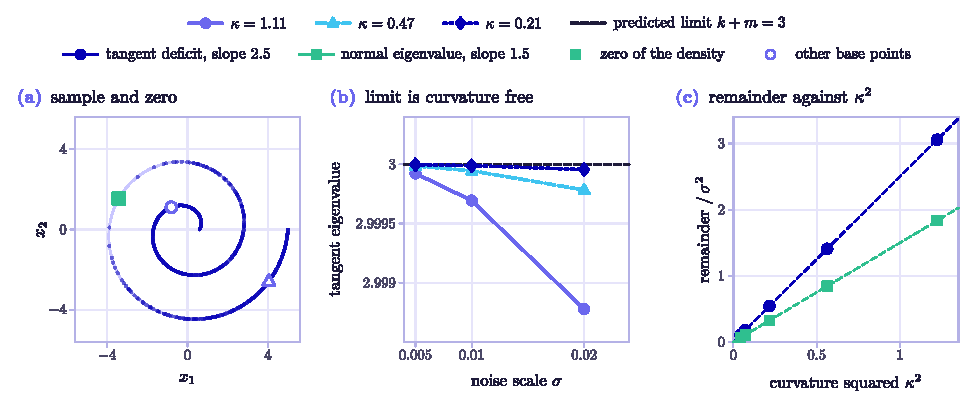
\includegraphics[width=\linewidth]{figures/spiral.pdf}
  \caption{A finite-type zero on a manifold with non-constant curvature.  (a) Fourteen hundred points drawn from the clean density \eqref{eq:spiral-density} for the zero at the filled square, with the manifold itself drawn as a faint guide.  The samples thin to nothing around that point, which is the feature the theorem is about.  The hollow circle and triangle mark two of the other tested base points; each carries its own density vanishing there, so each would empty a different part of the arc.  Both axes use the same scale, so the spiral keeps its true shape.  (b) The tangent Rayleigh quotient against noise scale at the three curvatures given in the legend, all converging to the predicted $k+m=3$ shown dashed, at rates that differ.  (c) The remainder at $\sigma=5\times10^{-3}$ against $\kappa^2$, with the dashed reference lines of slope $2.5$ for the tangent deficit and $1.5$ for the normal eigenvalue.  The limit does not depend on curvature; only the $O(\sigma^2)$ remainder does.}
  \label{fig:spiral}
\end{figure}

\section{Experimental details and numerical checks}
\label{app:experiments}

This appendix records the protocol of the population, finite-sample, and
exact-linearization experiments and of the trained-denoiser and end-to-end
optimization experiments.

\paragraph{Circle quadrature.}
We use a periodic uniform grid of $200{,}001$ points on $[-\pi,\pi)$ for the
spectrum experiment and $120{,}001$ points for each crossover curve.  The
right endpoint is excluded, so the same circle point is not counted twice.
At query angle $\alpha$, unnormalized weights are
\[
  w_j=
  \rho(\theta_j)
  \exp\!\left(
  -\frac{1-\cos(\theta_j-\alpha)}{\sigma^2}
  \right).
\]
After subtracting the largest log-kernel value for numerical stability, the
weights are normalized and the $2\times2$ posterior covariance is computed.
Projecting it onto the tangent and normal vectors at $\alpha$ and
dividing by $\sigma^2$ gives the plotted link blocks.  At the symmetric center
these blocks are eigenvalues.  At a moving query the cross block is generally
nonzero, so Figure~\ref{fig:spatial} labels the tangent quantity as
a Rayleigh quotient.

At the smallest plotted noise $\sigma=0.015$, the tangent eigenvalues for
$r=0,1,2,4$ are respectively
\[
  0.999887,\quad 2.999325,\quad 4.998312,\quad 8.994937,
\]
against predicted limits $1,3,5,9$.  The corresponding normal eigenvalues are at most $1.02\times10^{-3}$.  The same sweep also exhibits the rate in \eqref{eq:hlimit} rather than only its limit.  Regressing $\log|{\lambda_1(H_\sigma)-(k+m)}|$ on $\log\sigma$ over the small-noise end of the grid gives slope $2.000$ for each of $r=0,1,2,4$, and the deviations divided by $\sigma^2$ settle at $0.5000$, $3.0002$, $7.5004$, and $22.5013$.  On this family the observed constants agree with $(m+1)(m+2)/4$ to four digits, with $m=2r$.

\paragraph{Crossover accuracy.}
Across all plotted floor ratios and noise levels, the maximum absolute deviation from
$(\lambda+3/2)/(\lambda+1/2)$ is $3.01\times10^{-2}$ and the median deviation is $3.19\times10^{-3}$.  For the spatial boundary layer, the maximum absolute deviation from
$(a^4+3)/(a^2+1)^2$ is $3.01\times10^{-2}$ and the median is
$2.59\times10^{-3}$.  The largest errors occur at the largest noise, consistent with curvature corrections.

\paragraph{Normal offsets.}
The experiments plotted in Figures~\ref{fig:spatial} and \ref{fig:landing-error} query on the manifold, that is at $b=0$.  To check Theorem~\ref{thm:normal-boundary} at genuinely nonzero normal offset we evaluate the same circle quadrature at
$y=(1+\sigma b)(\cos\sigma a,\sin\sigma a)$, whose rescaled tangential and normal
coordinates are $a$ and $b$.  Table~\ref{tab:normal-offset} reports the tangent
block against its predicted limit $C_a=(a^4+3)/(a^2+1)^2$, the smaller
eigenvalue of $H_\sigma$ divided by $\sigma^2$, and the normal-only landing
error divided by $\sigma^2$.  Three predictions are visible.  The tangent-block
deviation divided by $\sigma$ is constant in $\sigma$, so that block is
$C_a+O(\sigma)$ as stated.  The limit does not depend on $b$: at $a=1$ both
$b=0$ and $b=1.3$ approach $1$, which is the uniformity in the normal
coordinate.  Finally $\lambda_2/\sigma^2$ and the landing error over $\sigma^2$
both converge, confirming $\lambda_{k+1}=O(\sigma^2)$ and the $O(\sigma^2)$
landing bias, and the landing limit does depend on $b$, as
\eqref{eq:normal-boundary-landing} requires through the term
$U_p\{\Lambda_a^\top b-S_ba\}$.

\begin{table}[!htbp]
  \centering
  \caption{Circle quadrature at nonzero normal offset, checking Theorem~\ref{thm:normal-boundary}.  The deviation column is $|U_p^\top H_\sigma U_p-C_a|/\sigma$, which is constant in $\sigma$ when the tangent block is $C_a+O(\sigma)$.}
  \label{tab:normal-offset}
  \small
  \begin{tabular}{@{}rrrrrrr@{}}
    \toprule
    $a$ & $b$ & $\sigma$ & $U_p^\top H_\sigma U_p$ & $C_a$
      & deviation$/\sigma$ & landing$/\sigma^2$ \\
    \midrule
    $0.0$ & $0.0$ & $0.020$ & $2.99880$ & $3.00000$ & $0.060$ & $1.500$ \\
    $0.0$ & $0.0$ & $0.005$ & $2.99992$ & $3.00000$ & $0.015$ & $1.500$ \\
    $1.0$ & $0.0$ & $0.020$ & $0.99967$ & $1.00000$ & $0.017$ & $0.500$ \\
    $1.0$ & $0.0$ & $0.005$ & $0.99998$ & $1.00000$ & $0.004$ & $0.500$ \\
    $1.0$ & $1.3$ & $0.020$ & $0.96200$ & $1.00000$ & $1.900$ & $0.808$ \\
    $1.0$ & $1.3$ & $0.005$ & $0.99031$ & $1.00000$ & $1.937$ & $0.817$ \\
    $-0.8$ & $1.3$ & $0.020$ & $1.21816$ & $1.26770$ & $2.477$ & $0.876$ \\
    $-0.8$ & $1.3$ & $0.005$ & $1.25508$ & $1.26770$ & $2.523$ & $0.898$ \\
    $2.0$ & $-1.1$ & $0.020$ & $0.77537$ & $0.76000$ & $0.769$ & $0.941$ \\
    $2.0$ & $-1.1$ & $0.005$ & $0.76383$ & $0.76000$ & $0.766$ & $0.930$ \\
    \bottomrule
  \end{tabular}
\end{table}

\paragraph{Exact optimization linearization.}
For $C_q=\diag(c,1)$ with $c=m+1$, the four tangent update matrices in
Figure~\ref{fig:conditioning} are
\[
  C_q(I-\gamma C_q),\qquad C_q(I-\gamma I),\qquad
  I-\gamma C_q,\qquad I-\gamma I.
\]
The stable interval of the raw inner-and-outer update is
$((c-1)/c^2,(c+1)/c^2)$ and has width $2/c^2$.  The inner-only interval is
$(1-1/c,1+1/c)$, and the raw-additive interval is $(0,2/c)$; both have width
$2/c$.  The doubly calibrated inner-step-and-normal-only-landing map has
interval $(0,2)$.  The plotted curves are
their exact spectral radii rather than simulated trajectories.  Each method
is evaluated over its own step-size range.

\paragraph{Finite-sample KDE.}
Samples from $\rho(\theta)=(1-\cos\theta)/(2\pi)$ are generated by exact rejection sampling from a uniform proposal, with acceptance probability $(1-\cos\theta)/2$.  For every seed we reuse prefixes of one sample stream at
$N\in\{20{,}000,80{,}000,320{,}000\}$ and evaluate \eqref{eq:empirical-kde} at
$\sigma\in\{0.035,0.05,0.075,0.11,0.16\}$.  We use $48$ fixed consecutive seeds,
$20260819$ through $20260866$.  For each $\sigma$, deterministic quadrature
first computes the finite-noise population reference $H_\sigma$.  We then record
\[
  \|\widehat H_N-H_\sigma\|_\op,\qquad
  \|\mathcal P_1(\widehat H_N)-\mathcal P_1(H_\sigma)\|_\op,\qquad
  |\lambda_1(H_\sigma)-3|,
\]
as separate sampling, subspace, and finite-$\sigma$ quantities.  The exact
population top eigenvalues across the plotted noise levels are respectively
$2.99632,2.99250,2.98310,2.96359,$ and $2.92269$.  Rounded-order success means
$\operatorname{round}(\lambda_1(\widehat H_N)-1)=2$.  Figure~\ref{fig:kde}
shows medians and interquartile ranges for the filled operator-error markers,
median-only open projector-error markers, and Wilson $95\%$ intervals for this
binomial success rate.  Since prefixes from a replication
are nested and effective sample size is itself random, the pooled display is
descriptive; no independence across plotted cells or universal
$\mathrm{ESS}^{-1/2}$ law is claimed.

\paragraph{Learned denoisers.}
Each denoiser is a residual MLP with two tanh hidden layers of
width $96$, and all of its parameters are trained.  Its inputs are the scaled
noisy vector and a normalized
$\log\sigma$ coordinate.  If $r_\theta(y,\sigma)$ is the network output, then
\[
  D_\theta(y,\sigma)=y+\sigma r_\theta(y,\sigma),
  \qquad
  \ell(\theta)=
  \E\left\|r_\theta(Y,\sigma)-\frac{X-Y}{\sigma}\right\|^2.
\]
The three circle noise levels are $0.08,0.12,0.18$, and the plane levels are
$0.12,0.18,0.25$; during training $\sigma$ is drawn uniformly from these three
values rather than from a continuous range, and the same three values are used
for evaluation.  Training pairs are generated afresh at every step from the
exact sampler, so there is no fixed finite training set and no repetition, and
the learned-model error therefore reflects approximation and optimization error
rather than memorization of a sample.  The scaled noisy input is $y$ divided by
$1.25$ for the circles and by $0.85$ for the plane.  We optimize every parameter for $3500$ Adam steps with batch
size $768$, cosine-decayed learning rate from $2.5\times10^{-3}$ to
$2.5\times10^{-4}$, weight decay $2\times10^{-6}$, and gradient-norm clipping
at $8$.  Validation uses $20{,}000$ fresh pairs.

To increase query coverage without changing the population regression
function, each minibatch mixes $15\%$ unweighted samples with $85\%$ samples
resampled from an eight-times-larger pool according to the strictly positive
weight $w(y)=\exp\{-\|y-c\|^2/(2r^2)\}+10^{-4}$, normalized over the pool, which
depends only on $Y$; here $c$ is the evaluation point and $r$ the query radius
below.  Multiplication of the joint density by a
function of $Y$ leaves $\mathbb E[X\mid Y=y]$ unchanged wherever the weight is
positive.  The query radii are $0.22$ for the circle and $0.38$ for the plane.
This resampling changes finite-model optimization but not the population
conditional target.

The residual MLP has an analytic input Jacobian obtained by the chain
rule through both tanh layers.  We form
$\widehat H_\theta=\operatorname{sym}(\nabla_yD_\theta)$, then evaluate the raw
matrix, its hard top-$k$ projector, and $\Phi_{0.25}((\widehat H_\theta)_+)$.
For the regime diagnostic of Table~\ref{tab:calibration-regime} we also record,
in the true tangent frame at the evaluation point, the coupling block
$\|P^\perp\widehat H_\theta P\|_\op$ and the computed separation
$\delta(\widehat H_\theta)$ of \eqref{eq:computed-separation}, obtained from the
two compressions $U^\top\widehat H_\theta U$ and
$U_\perp^\top\widehat H_\theta U_\perp$, where the columns of $U_\perp$ are an
orthonormal basis of the normal space.  A
centered finite-difference audit with step $10^{-6}$ and seed $2026081998$
found an operator-norm Jacobian discrepancy of $1.69\times10^{-10}$.  The plane population reference is evaluated in closed form rather than by
quadrature: homogeneity of $q_4$ makes the tilt scale free, so
$H_\sigma(p)=\tfrac{s^2}{s^2+\sigma^2}UC_qU^\top$ with $s=0.35$ and
$C_q=\diag\{(m+1+\epsilon)/(1+\epsilon),(1+\epsilon(m+1))/(1+\epsilon)\}$ for
$m=4$ and anisotropy $\epsilon=0.1$, whose trace is $k+m=6$.  The fixed
plane frame is obtained by seeded QR in $\R^{16\times2}$.  Its latent
distribution is sampled exactly as a mixture of polynomially tilted
Gaussians; a $4{,}000{,}000$-draw check with seed $2026081997$ obtained second
moments $(0.568106,0.167006)$ against analytic values $(0.567955,0.167045)$, with
maximum relative error $2.67\times10^{-4}$.

There are $12$ independent base replications indexed by seeds $2026081900$
through $2026081911$.  Each replication trains one model for each of the three
problems, for $36$ denoisers total; the plane frame seed is $2026081901$, and the paired
bootstrap seed is $2026081999$.  Shaded figure bands show interquartile ranges,
not confidence intervals.  The two quoted paired intervals use $20{,}000$
percentile-bootstrap resamples of the within-seed raw-minus-hard differences.

\paragraph{Learned optimization.}
For the circle we minimize $f(x)=\|x-(1,0)\|^2/2$ from angle $0.55$ for $35$
steps; for the plane we minimize $f(x)=\|U^\top x\|^2/2$ from latent
coordinate $(0.40,-0.32)$ for $30$ steps.  Both targets are ambient critical
points, as required by Corollary~\ref{cor:local-invariant}.  For each method,
we sweep $20$ circle step sizes from $0.05$ to $1$ and $24$ plane step sizes
from $0.05$ to $1.2$.  Each sweep is run at all three noise levels the
corresponding denoiser was trained on, namely $0.08,0.12,0.18$ for the circle and
$0.12,0.18,0.25$ for the plane, which requires no additional training because the
networks are noise conditional.  Figure~\ref{fig:learned-optimization} plots
the middle level of each problem, $\sigma=0.12$ and $\sigma=0.18$, and the
noise dependence of the achieved floor is reported in
Section~\ref{sec:experiments}.
The raw method uses $\widehat H_\theta$ in the inner step and
$D_\theta$ as the outer landing.  The inner-only method replaces the first by
$\mathcal P_k(\widehat H_\theta)$ but retains raw landing.  SC-DRGD uses the
hard projector in both the tangent step and the normal-only landing.  Oracle
Riemannian gradient descent is included as a deterministic reference.  We
report the projected objective gap
$F(x_t)-F(p)=f(\pi(x_t))-f(p)$ and distance to the manifold for every
iteration, seed, method, and step size; for the affine plane, $F=f$.  Values
are clipped only when drawing the log-scale figure.

\paragraph{Compute.}
The reported run used the full training configuration with Python 3.12.13 and
NumPy 2.3.5 on an arm64 CPU without an accelerator; its recorded
wall-clock time was $169.8$ seconds.
